\section{Control Plane and Orchestration layers in data centers}
After examining the main overlay technologies, the following section focuses on the control plane and orchestration layers that enable communication, automation, and coordination across virtualized network infrastructures in modern data centers.

\subsection{Control Plane}

In traditional networking, the control plane is responsible for maintaining topology information and making forwarding decisions, which are then executed by the data plane. Within virtualized data center environments, the control plane extends this function to manage logical networks that span multiple hypervisors and physical domains. It provides the intelligence necessary to synchronize routing, addressing and policy enforcement across distributed systems.

A key challenge lies in maintaining consistency between logical and physical network states. Software-Defined Networking (SDN) introduces a logically centralized control architecture that decouples the control and data planes, improving programmability and abstraction of network resources. The SDN controller exposes well-defined application programming interfaces (APIs) to upper layers, allowing network resources to be represented as logical entities independent of the underlying transport technology. This abstraction supports the creation of multiple virtual tenant networks (VTNs), each with its own control-plane instance.

In practice, SDN controllers such as OpenDaylight or Floodlight are instantiated within data centers as virtual functions, enabling flexible and isolated control per tenant. The virtualization of control functions, as virtual SDN controllers, reduces configuration time and facilitates high availability through rapid redeployment across data-center servers. The controller’s role is central in dynamically programming virtual resources, maintaining topological state, and establishing forwarding paths via protocols such as OpenFlow or NETCONF/YANG.

\subsection{Network Orchestration}

Network orchestration refers to the coordinated management and automation of network and compute resources to ensure that complex infrastructures operate as a cohesive system. It provides a unified control layer that translates high-level service requirements into automated configuration and provisioning actions across physical and virtual domains. Unlike traditional network management, which often focuses on device-level operations, orchestration operates at a service level, ensuring that the entire network adapts dynamically to application and user demands.

In modern data centers, orchestration integrates the deployment, configuration, scaling and monitoring of network services into a single, policy-driven workflow. It enables consistency and automation by defining service intent through abstract models rather than manual commands. These models describe what the network should achieve, such as bandwidth, latency or security constrains, while the orchestration system determines how to implement them using available resources. Through well-defined interfaces and APIs, orchestration platforms interact with underlying control planes, such as SDN controllers or virtualization managers, to enforce the desired network behaviour automatically.

\begin{wrapfigure}{r}{0.4\textwidth}
    \vspace{-15pt}
    \centering
    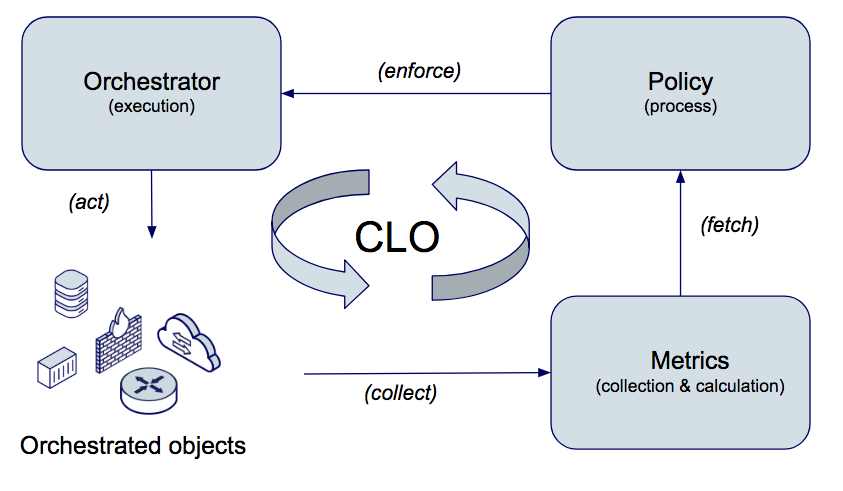
\includegraphics[width=\linewidth]{Figures/orchestration.png}
    \caption{Closed Loop Orchestration. \cite{orchestration}}
    \label{closedLoop}
    \vspace{-5pt}
\end{wrapfigure}

A key characteristic of network orchestration is automation through a closed loop (CLO), illustrated in Figure \ref{closedLoop},where monitoring and analytics continuously evaluate the operational state of the infrastructure and trigger corrective actions when deviations occur. This allows the network to maintain compliance with predefined service-level objectives without human intervention, contributing to the development of self-optimizing infrastructures.

In virtualized data centers, orchestration systems coordinate with control-plane mechanisms, such as SDN controllers and virtual infrastructure managers, to deploy and adapt network services. The orchestration layer operates at a higher level of abstraction, managing service intent and lifecycle, while the control plane translates these policies into real-time configurations. This separation improves scalability, consistency and agility, allowing data centers to deliver automated, policy-driven network services across diverse physical and virtual environments.

\subsection{Integration of Control and Orchestration layers}

The integration between orchestration and control layers is essential to achieve end-to-end automation and operational agility in virtualized data centers. As explored in the previous subsections, the control plane is responsible for real-time network configuration, path computation and enforcement of forwarding policies, while the orchestration layer operates at a higher level of abstraction, coordinating multiple control entities to deliver coherent and policy-driven service management. This hierarchical relationship, illustrated in Figure \ref{layerIntegration}, allows service intent, defined at the orchestration layer, to be systematically enforced by the control plane across heterogeneous infrastructures.

\begin{figure}[H]
    \centering
    \vspace{-5pt}
    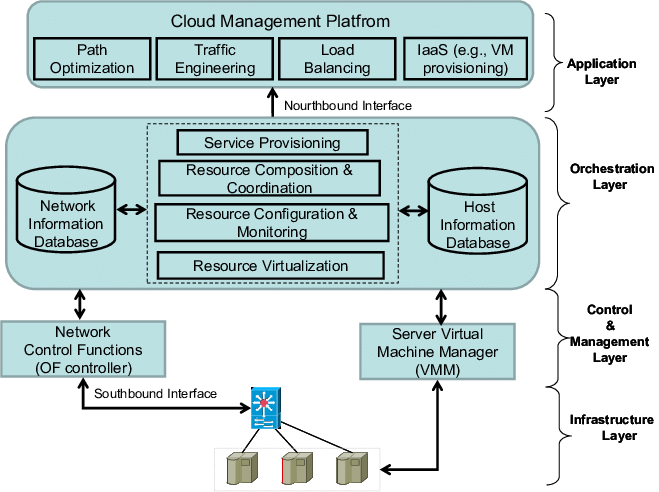
\includegraphics[width=0.5\linewidth]{Figures/layerIntegration.png}
    \caption{Hierarchical integration between orchestration, control and infrastructure layers. \cite{adami2015orchestrator}}
    \label{layerIntegration}
\end{figure}
\newpage
The communication between the two layers is typically implemented through standardized APIs and data models, such as REST, NETCONF/YANG or TOSCA, which ensure interoperability across multiple vendors and technologies. Through this layered coordination, orchestration systems gain visibility into network state and can trigger adjustments via the control plane, ensuring alignment between service intent and operational reality.

The result is a scalable and adaptive control architecture in which orchestration defines what the network should achieve, and the control plane determines how to realize it. This separation of concerns enables data centers to operate as automated, policy-driven environments capable of dynamic optimization and rapid service deployment.